% Draft layout only. Replace acmart with the official MLSys 2027 style after
% the conference publishes its submission package; do not assume the 2026
% style is unchanged.
\documentclass[sigconf,review,anonymous]{acmart}

\usepackage{graphicx}
\usepackage{xcolor}
\usepackage{booktabs}

\title{Priority Starts Before the GPU:\\
Cross-Stage Service Scheduling for Multimodal LLM Serving}

\begin{document}

\begin{abstract}
Multimodal LLM requests consume service before they reach the GPU: videos must
be fetched, decoded, sampled, and transformed into model inputs. Existing
engine schedulers account only for requests that have completed this work.
Consequently, neither tenant fairness nor foreground priority composes across
the independently admitted CPU-preparation and GPU-inference stages. We
present a cross-stage scheduler that maintains weighted virtual service for
each tenant at both admission boundaries, applies foreground priority within
the selected tenant, bounds admitted media work, and ages background requests.
It retains asynchronous overlap and leaves active decoding non-preemptive. In
24 matched, error-free trials, adding cross-stage foreground priority to a
virtual-service baseline reduces foreground mean completion latency from
176.00 to 44.72 seconds (3.94$\times$) while preserving throughput (0.226
versus 0.230 requests/s) and nearly the same worst-to-best tenant slowdown
(1.15$\times$ versus 1.19$\times$). A corrected native-vLLM raw-video control
independently shows that bounded media priority improves urgent mean TTFT by
1.66$\times$ without changing accuracy or throughput.
\end{abstract}

\maketitle

\section{Introduction}

ML serving platforms increasingly share accelerators among tenants and among
requests with different latency objectives. A tenant may issue synchronous
foreground queries together with offline evaluation, indexing, or batch
analysis. Existing inference schedulers can allocate GPU service among
tenants or accelerate foreground work---but only after a request enters the
engine queue.

Multimodal requests complicate this model. Before a video question reaches
the inference engine, the serving pipeline may need to open the video,
demultiplex its container, select temporal positions, seek to keyframes,
decode and resize frames, and construct a model-ready input. These operations
consume CPU, storage, memory bandwidth, and decoder capacity. They are also
commonly managed by a media-preparation queue separate from the inference
engine.

This separation creates a more general gap than a missing priority queue.
Service objectives enforced at the GPU do not automatically hold end to end.
A tenant can receive an equal GPU share yet wait disproportionately for CPU
preparation; a foreground request can be ordered first at the engine yet
remain behind background decoding upstream. By the time an engine policy
takes effect, the delay and interference have already occurred.

We call the priority instance of this failure \emph{upstream priority
inversion}: a foreground multimodal request is delayed by background work in
a stage preceding the priority-aware model engine. Figure~\ref{fig:design-overview}
illustrates this case. More broadly, the failure is one of \emph{cross-stage
service accounting}: independently admitted stages can each appear locally
well scheduled while violating the application's end-to-end ordering and
isolation objectives.

\begin{figure*}[t]
    \centering
    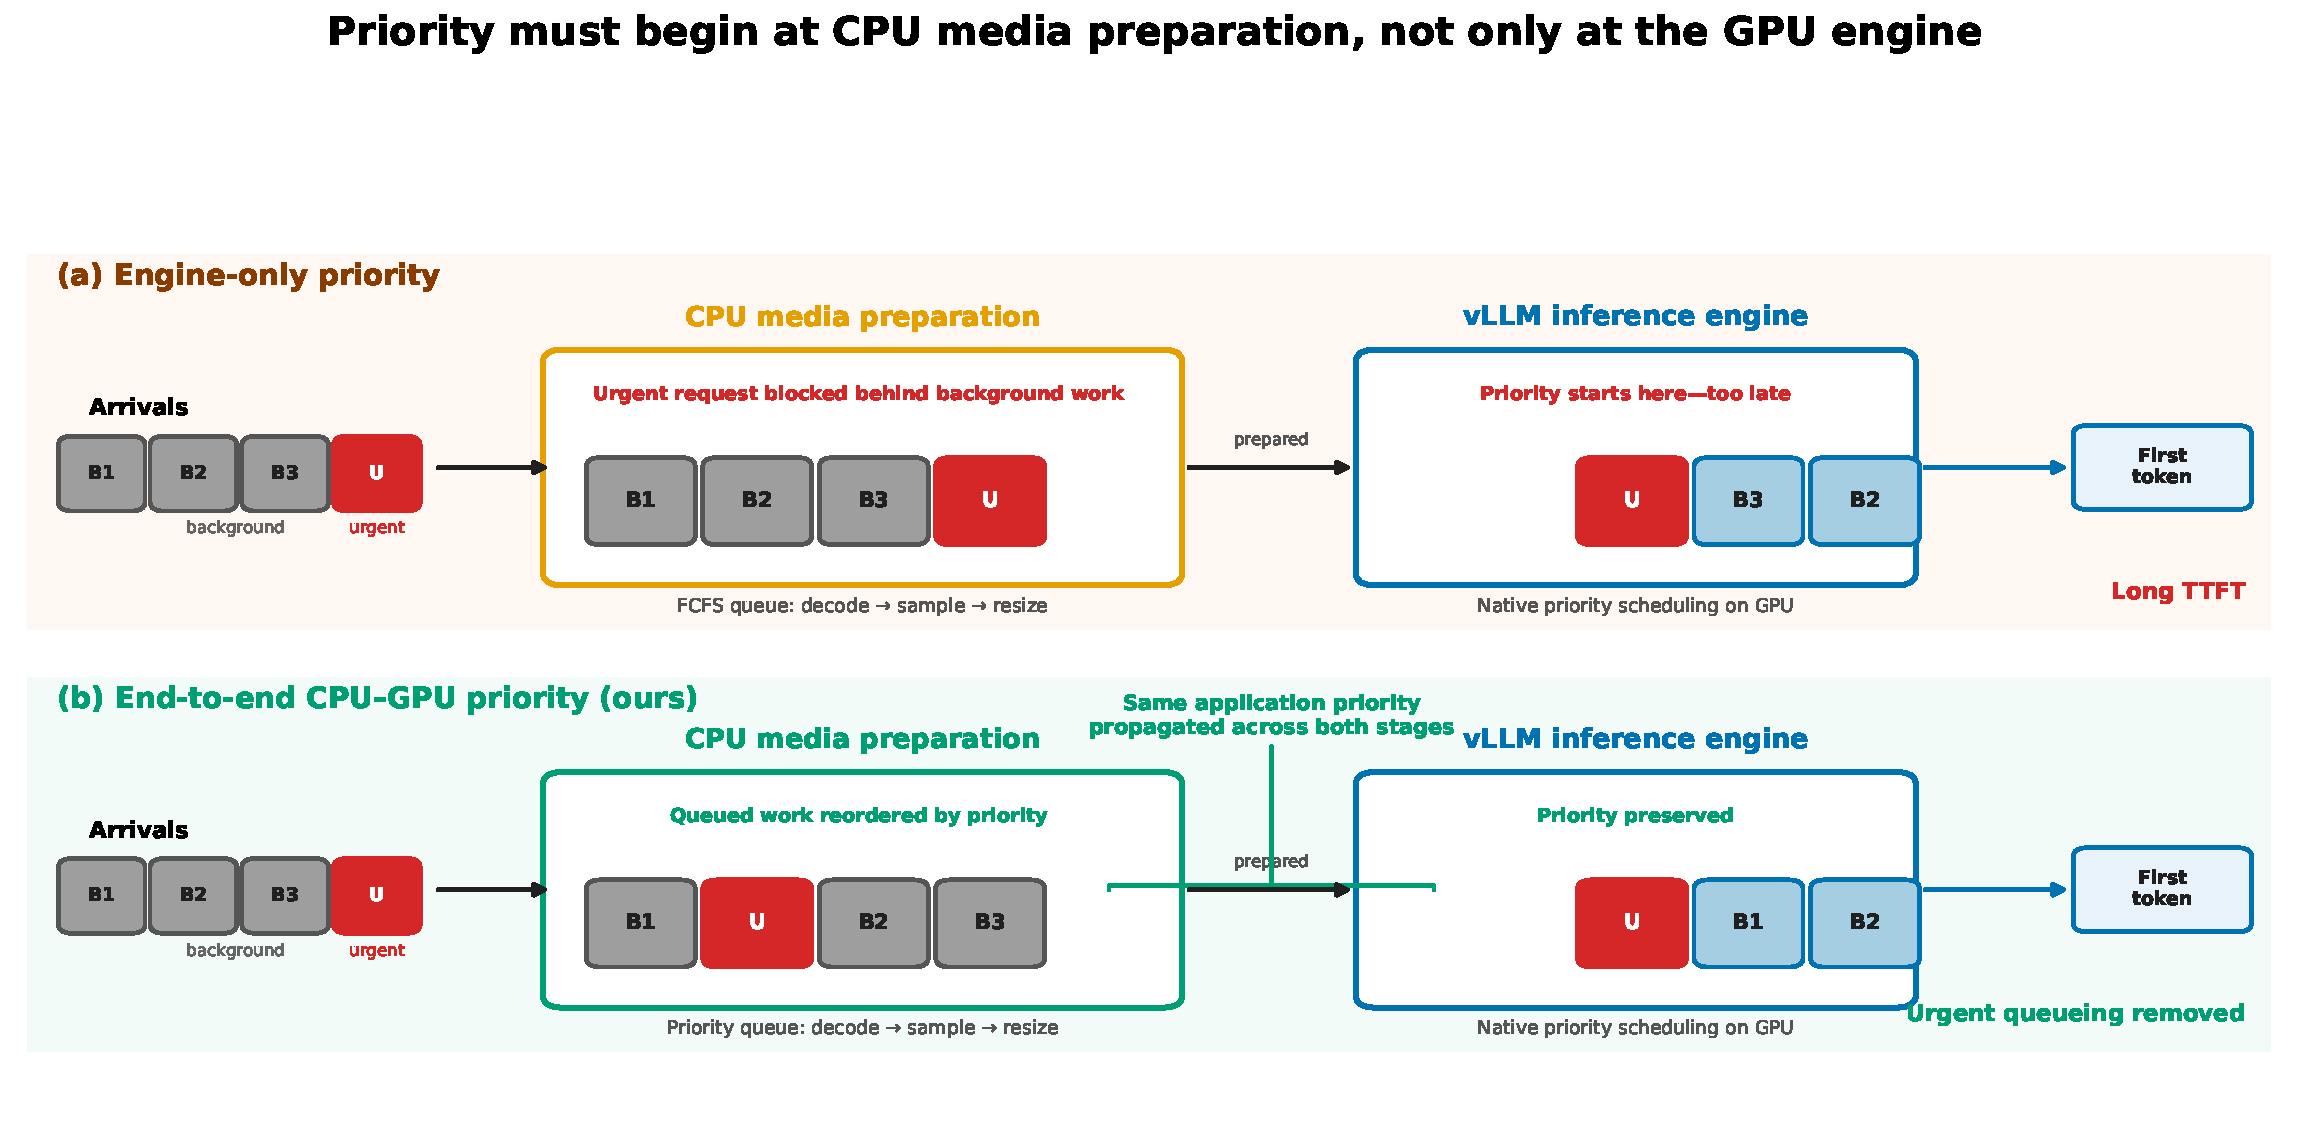
\includegraphics[width=\textwidth]
        {figures/cpu_end_to_end_priority_diagram.pdf}
    \caption{\textbf{Upstream priority inversion and our end-to-end design.}
    Both configurations use native vLLM priority. With FCFS media
    preparation, an urgent request remains blocked behind queued background
    decoding before becoming visible to vLLM. End-to-end priority applies the
    same application-assigned priority to queued CPU preparation and GPU
    inference. Active preparation remains non-preemptive.}
    \Description{Two timelines compare engine-only priority with end-to-end
    priority. In the first, an urgent request waits behind background video
    preparation before reaching vLLM. In the second, it overtakes queued but
    not executing background preparation and reaches vLLM earlier.}
    \label{fig:design-overview}
\end{figure*}

\paragraph{Upstream queueing can dominate responsiveness.}
We demonstrate this problem using Qwen2.5-VL-7B-Instruct served by vLLM. Our
corrected native raw-video experiment contains 63 low-priority background
requests followed by 16 urgent requests and uses verified per-request budgets
from 8 to 128 frames. Both configurations retain vLLM's asynchronous frontend
and native engine priority. Adding bounded, priority-aware media admission
reduces urgent mean TTFT from 53.88 to 32.47 seconds, a 39.7\% reduction or
1.66$\times$ speedup, with no errors and effectively unchanged throughput.

\paragraph{Asynchrony is useful but does not define service order.}
Native asynchronous processing overlaps URL fetching, decoding,
preprocessing, and inference, and is therefore an important high-performance
baseline. However, concurrency alone neither bounds how much media work is
admitted nor determines which waiting job should receive CPU and decoder
capacity first. Our change preserves this overlap but inserts a bounded
priority admission point before fetching and decoding. Urgent requests can
therefore overtake queued background work, while work already executing
remains non-preemptive.

\paragraph{Scaling resources does not remove an ordering failure.}
Faster GPUs and additional model replicas increase inference capacity but do
not necessarily increase the capacity of a shared media-preparation tier.
Likewise, additional CPU workers reduce queueing only until CPU, storage, and
memory-bandwidth contention become limiting. More capacity also does not
express which queued request is urgent. Even with 16 preparation workers,
priority-aware preparation reduces urgent mean TTFT from 87.62 to 33.48
seconds with effectively unchanged throughput.

\paragraph{Our proposal: cross-stage service scheduling.}
We separate two decisions that a production scheduler must not conflate.
First, weighted virtual service chooses which tenant should receive the next
unit of preparation or inference admission. Second, within that tenant,
foreground priority chooses among its queued requests. The same hierarchy is
applied before non-preemptive media preparation and before inference. Bounded
admission keeps unstarted work reorderable, while aging guarantees that old
background work eventually progresses. Thus one tenant cannot obtain another
tenant's share merely by labeling every request foreground.

\paragraph{Results.}
Across four matched seeds and six policies (24 error-free runs), tenant
fairness alone leaves foreground mean completion latency at 176.00 seconds.
Adding priority within each tenant reduces it to 44.72 seconds
(3.94$\times$), raises 60-second attainment from 0.0\% to 77.1\%, and
preserves both throughput and tenant isolation. Globally strict priority is
faster (37.18 seconds) but worsens the worst-to-best tenant slowdown ratio
from 1.19$\times$ to 2.52$\times$. These results expose a useful operating
point between foreground latency and cross-tenant isolation rather than
hiding the cost in background work.

This paper makes three contributions:

\begin{enumerate}
    \item \textbf{Cross-stage scheduling failure.}
    We show that engine-local priority and tenant fairness do not compose
    across independently admitted media-preparation and inference stages, and
    decompose end-to-end latency into the service and queueing at each stage.

    \item \textbf{Hierarchical cross-stage service accounting.}
    We design a work-conserving scheduler that selects tenants by weighted
    virtual service, orders foreground work within the selected tenant, bounds
    media admission, and ages background requests. It applies the same
    hierarchy at preparation and inference while retaining asynchronous
    overlap and non-preemptive decoding.

    \item \textbf{End-to-end evaluation.}
    We compare FCFS, strict priority, shortest-job-first, virtual-service
    tenant fairness, hierarchical tenant priority, and slowdown-aware service
    across matched workloads. We report completion latency and attainment,
    TTFT, throughput, tenant isolation, background progress, errors, and
    accuracy, together with CPU-worker and inference-replica sensitivity.
\end{enumerate}

\section{Background and Motivation}

\subsection{Multimodal Inference Pipeline}

Figure~\ref{fig:design-overview} shows the two independently queued stages in
a video-MLLM serving pipeline. A request contains a textual question and a
compressed video. The front end probes the video, selects temporal positions,
decodes and resizes frames, and constructs the multimodal model input. After
preparation, the request enters the model-serving engine, which applies its
multimodal processor, executes the vision encoder, prefills the language
model, and decodes the response. Engines such as vLLM support continuous
batching and priority scheduling for requests already admitted to the engine
queue~\cite{vllm}.

We decompose end-to-end TTFT as

\begin{equation}
T_{\mathrm{TTFT}} =
T_{\mathrm{prep\mbox{-}queue}} +
T_{\mathrm{prep\mbox{-}service}} +
T_{\mathrm{handoff\mbox{-}queue}} +
T_{\mathrm{engine\rightarrow token}}.
\end{equation}

The four terms represent time waiting for a media worker, time spent preparing
the video, time waiting for downstream admission, and engine execution until
the first token. Engine scheduling directly controls only work visible after
preparation; it cannot reorder a compressed video still waiting upstream.

\subsection{Contention During Media Preparation}

Concurrent video requests compete for CPU cores, storage bandwidth, memory
bandwidth, decoder state, and a finite pool of preparation workers. This tier
can become the bottleneck even when the GPU has spare capacity. Adding model
replicas increases downstream inference capacity but does not increase a
shared preparation pool. Increasing preparation workers improves capacity,
but workers eventually contend for shared host resources and still do not
encode urgency.

The problem also does not require every request to be individually expensive.
With every request restricted to four frames, priority-aware preparation
improves urgent TTFT by 2.50$\times$; at eight frames, the improvement reaches
4.15$\times$. At two frames, both policies perform similarly because the
preparation tier remains below capacity. The failure therefore arises from
aggregate contention and FCFS ordering, not merely from long videos.

\subsection{Upstream Priority Inversion}

Applications commonly assign priorities to distinguish interactive requests
from background work. A text-only request can proceed directly to engine
admission and benefit immediately from engine priority. A video request,
however, is invisible to the engine while its frames are being prepared.
Assigning different engine priorities to two video requests therefore does
not determine their preparation order. If preparation is FCFS, a
high-priority video can still reach the engine after a low-priority video.

This differs from inversion within the inference engine: the engine has no
visibility into or control over the blocked request. Engine scheduling can
improve latency after admission, but it cannot recover upstream time already
lost.

\subsection{Limitations of Existing Mitigations}

\paragraph{Engine-level scheduling.}
Priority, preemption, fair scheduling, chunked prefill, and
prefill--decode disaggregation operate on requests already visible to the
inference runtime~\cite{fastserve,andes,sarathiserve,distserve}. They do not
determine which compressed video an upstream preparation service decodes
next.

\paragraph{Inference scale-out.}
Additional GPU replicas alleviate engine contention but do not increase a
shared CPU preparation pool. Fully isolating urgent traffic would require
reserving both inference and preparation capacity, wasting resources whenever
urgent traffic is absent.

\paragraph{Faster preparation.}
Additional CPU workers, batched decoding, NVDEC, caching, and frame reduction
can reduce preparation service time. These optimizations are complementary to
scheduling: a faster FCFS decoder can still execute low-priority work before
an urgent request. Cold or unique videos also cannot depend on cached media.

\section{Design}
\label{sec:design}

Our scheduler is an external front end to a priority-aware inference engine.
It does not modify the model, video decoder, or GPU scheduler. Instead, it
closes the priority gap between request arrival and engine admission.

\subsection{Design Goals}

The design provides (1) weighted service isolation among tenants across both
CPU preparation and GPU admission, (2) foreground priority within each
tenant, (3) work conservation when a class or tenant is idle, (4) eventual
background progress, and (5) compatibility with an unmodified inference
engine. Active preparation remains non-preemptive, so a foreground request
may experience residual blocking from at most the tasks already running.

\begin{figure}[t]
    \centering
    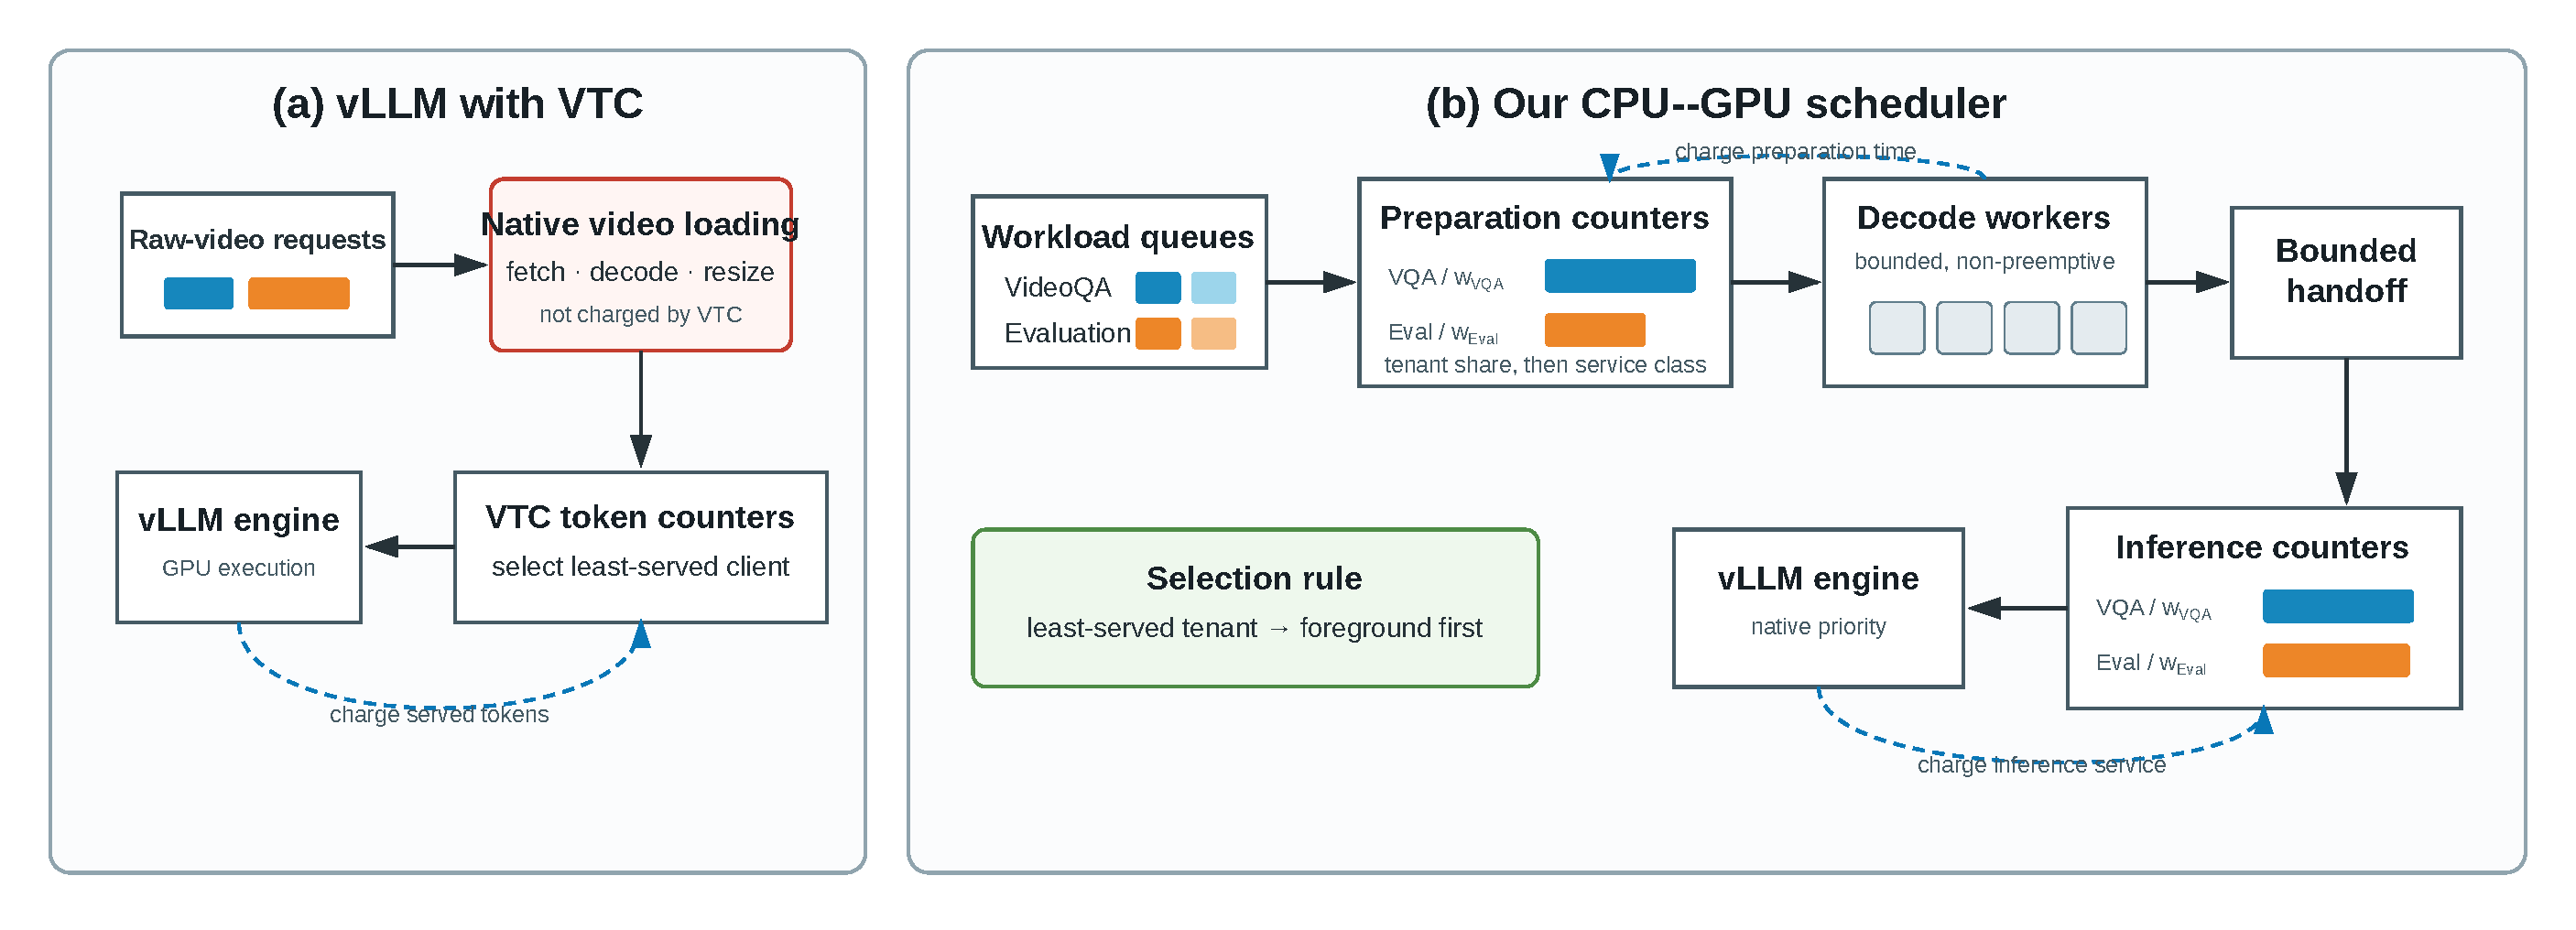
\includegraphics[width=\columnwidth]
        {figures/cross_stage_virtual_service_minimal.pdf}
    \caption{\textbf{Cross-stage virtual service.} Separate virtual-service
    counters account for tenant service at media preparation and inference
    admission. At each boundary, the scheduler first selects an underserved
    tenant and then applies foreground priority within that tenant.}
    \Description{A minimal block diagram shows tenant request queues feeding
    a CPU media-preparation scheduler and a GPU inference scheduler. Both
    schedulers consult per-tenant virtual-service counters.}
    \label{fig:cross-stage-service}
\end{figure}

\subsection{Request Metadata and Ordering}

Each request is represented as

\begin{equation}
r = \langle id_r, t_r, w_{t_r}, p_r, a_r, f_r, s_r \rangle,
\end{equation}

where $id_r$ is the identifier, $t_r$ is its authenticated tenant,
$w_{t_r}>0$ is that tenant's configured share, $p_r$ is the workload class,
$a_r$ is arrival time, $f_r$ is frame budget, and $s_r$ is an optional latency
objective. Smaller numerical values indicate higher within-tenant priority.
A video question is one multimodal request; its class applies to preparation
and subsequent inference, not independently to its text and video components.

The pending preparation queue uses

\begin{equation}
K(r) = (p_r, a_r, id_r),
\end{equation}

which enforces priority and deterministic FCFS order within a priority class.
The dispatcher admits work only when one of $W$ preparation workers is free.
Unlike immediately submitting every request to a FIFO thread pool, this
explicit pending queue keeps unstarted work visible and reorderable.

\subsection{Hierarchical Tenant and Workload Selection}

Strict global priority can protect foreground requests by transferring nearly
all delay to background tenants. Pure tenant fairness has the opposite
failure: it allocates equal service among tenants but cannot distinguish a
tenant's interactive query from its own batch work. We compose the two
objectives hierarchically rather than comparing incomparable priority labels
across tenants.

For each stage $x\in\{\mathrm{prep},\mathrm{engine}\}$, the scheduler tracks a
virtual-service counter $V_t^x$ for every active tenant. Dispatching estimated
service $\widehat{c}_r^x$ updates

\begin{equation}
V_{t_r}^x \leftarrow V_{t_r}^x +
\frac{\widehat{c}_r^x}{w_{t_r}}.
\end{equation}

When the operation completes, the estimate is reconciled with observed
service. At a free preparation worker or inference-admission slot, the
scheduler chooses the active tenant with the smallest $V_t^x$, then chooses
that tenant's highest-priority request, breaking ties by arrival order. A
newly active tenant joins at the current service frontier rather than at zero,
preventing it from receiving an artificial burst of service. This mechanism
is inspired by virtual-service fair queueing; it is not presented as a new
fair-queueing primitive. Its role is to extend service accounting across a
multimodal pipeline boundary that an engine-only policy cannot observe.

\subsection{Non-Preemptive Preparation}

Once a worker starts a request, it completes indexing, frame decoding,
resizing, and input construction. This avoids discarding partial work,
reconstructing decoder state, and restarting costly media operations. The
scheduler removes blocking from the queued backlog but does not preempt the
at-most-$W$ tasks already executing.

\subsection{Bounded Handoff and Engine Submission}

Prepared requests enter a bounded queue before vLLM submission. The bound
prevents the CPU tier from placing a large low-priority backlog in front of
the engine and preserves scheduling flexibility. When admitted to vLLM, a
request carries the same priority used during preparation:

\begin{equation}
\text{priority preparation}
\rightarrow \text{bounded handoff}
\rightarrow \text{priority inference}.
\end{equation}

vLLM remains responsible for continuous batching, KV-cache management, and
GPU execution.

\subsection{Optional Reserved Capacity}

When all workers are executing long background tasks, strict priority still
experiences residual non-preemptive blocking. With $W$ workers and reservation
$R$, at most $W-R$ workers may begin background preparation. Our primary
reserved configuration uses $W=4$ and $R=1$. Reservation strengthens urgent
protection but can leave capacity idle, so we evaluate it as an optional
policy rather than the default.

\subsection{Starvation Protection}

Continuous foreground traffic can delay background requests within a tenant.
After a configured waiting interval, an old background request is promoted to
the best priority currently queued for that tenant. Tenant selection remains
controlled by virtual service, so aging cannot consume another tenant's
share. Aging is a progress guardrail, not the source of the primary
foreground-latency improvement.

\section{Implementation}
\label{sec:implementation}

We implement the scheduler as an external Python serving front end. It
maintains explicit pending preparation and inference-admission queues, a
fixed-size pool of non-preemptive workers, per-stage tenant virtual-service
counters, and a bounded queue for prepared requests. FCFS and strict-priority
modes retain native vLLM priority. For policies that own both admission
boundaries, the front end submits uniformly prioritized requests after making
the hierarchical tenant and workload decision itself. The implementation
requires no changes to vLLM, the model, or the video decoder.

The runner records request arrival, preparation start and completion, engine
submission, first token, completion, selected replica, prediction, and error
status. These events allow us to attribute end-to-end TTFT to preparation
queueing, preparation service, handoff queueing, and inference.

\section{Evaluation Methodology}
\label{sec:evaluation-methodology}

Our evaluation asks:

\begin{enumerate}
    \item Do engine-local tenant fairness and workload priority preserve their
    objectives across CPU preparation and GPU inference?
    \item Can hierarchical cross-stage scheduling protect foreground work
    without surrendering tenant isolation or throughput?
    \item How does the policy compare with FCFS, global priority,
    shortest-job-first, pure tenant fairness, and slowdown-aware service?
    \item Can additional preparation workers or inference replicas eliminate
    the cross-stage failure without coordinated admission?
    \item How do frame budget, arrival pattern, video duration, and decoding
    strategy affect the result?
\end{enumerate}

\subsection{Testbeds and Default Configuration}

Our experiments use NVIDIA A40 GPUs. Each GPU hosts one independent vLLM
replica serving Qwen2.5-VL-7B-Instruct. Unless varied, each trial uses one
replica and one shared CPU media-preparation tier. Preparation-worker,
reservation, and decoding ablations also use a server with two Intel Xeon Gold
6130 processors (32 physical cores and 64 hardware threads).

\begin{table}[t]
    \centering
    \small
    \caption{Default experimental configuration.}
    \label{tab:default-config}
    \begin{tabular}{ll}
        \toprule
        Component & Configuration \\
        \midrule
        Model & Qwen2.5-VL-7B-Instruct \\
        GPU & NVIDIA A40 \\
        Inference engine & vLLM, native priority \\
        Model replicas & 1 unless varied \\
        Maximum model length & 16,384 tokens \\
        Maximum generated tokens & 32 \\
        GPU memory utilization & 0.85 \\
        Prefix caching & Disabled \\
        Multimodal processor cache & Disabled \\
        Preparation workers & 4 unless varied \\
        VLM concurrency & 4 per replica \\
        Prepared-queue depth & 32 \\
        Maximum decoded side & 448 pixels \\
        Maximum input pixels & 100,352 \\
        Default backend & CPU frame seeking \\
        Request timeout & 1,800 seconds \\
        \bottomrule
    \end{tabular}
\end{table}

VLM concurrency is the maximum number of outstanding client requests sent to
each vLLM replica; it is not the engine's GPU batch size. We disable prefix and
multimodal processor caching so repeated requests do not bypass preparation.
Before each trial, we wait until vLLM reports no running or waiting requests.

\subsection{Workloads and Arrivals}

We evaluate a 249-question video-QA pool drawn from EgoSchema, NExT-QA,
VRBench, STAR, and LVBench. Each main trace contains 64 low-priority
background requests (priority 10) and 16 urgent requests (priority 0).
Background requests represent offline indexing, evaluation, captioning, or
batch analysis; urgent requests represent interactive queries.

We evaluate six arrival configurations: one burst, one evenly staggered
stream, and randomized exponential arrivals at 0.25, 0.5, 0.75, and 1.0
requests per second. Urgent traffic begins at 1, 10, 30, or 60 seconds. Five
seeds produce $6\times4\times5=120$ matched traces. Every policy receives the
same questions, videos, arrival times, frame budgets, and seed.

The main traces use duration-aware budgets of 8, 16, 32, 64, and 128 frames.
Controlled experiments use fixed budgets of 2, 4, 8, and 128 frames to
separate scheduling effects from large per-request frame counts.

\subsection{Policies and Capacity Baselines}

We compare:

\begin{itemize}
    \item \textbf{Engine-only priority}: FCFS CPU preparation and native vLLM
    priority;
    \item \textbf{End-to-end priority}: the same application priority at CPU
    preparation and vLLM; and
    \item \textbf{Priority with reserved capacity}: end-to-end priority with
    one of four workers protected from background admission.
\end{itemize}

All policies use native vLLM priority, so engine-only versus end-to-end
isolates the scheduling of the upstream stage. Capacity comparisons vary
preparation workers over 2, 4, 8, and 16 and inference replicas over 1, 2, and
4. Fixed-load replica experiments keep requests constant; proportional-load
experiments scale offered work from 80 to 160 and 320 requests while retaining
four shared preparation workers.

The multi-tenant experiment additionally compares six external policies on
identical traces: FCFS; globally strict priority; shortest-job-first using a
predicted service cost; tenant fairness, which selects the least-served tenant
and then its oldest request; tenant-fair priority, which selects the
least-served tenant and then its foreground request; and fair slowdown, which
selects the least-served tenant and then the request with greatest predicted
completion slowdown. The tenant-fair policies use uniform engine priorities
because the external scheduler owns ordering at both admission boundaries.
Our tenant-fair baseline is VTC-inspired and is not claimed to be a faithful
reproduction of VTC's token-level engine scheduler.

\subsection{Metrics and Statistical Methodology}

The primary metrics are foreground end-to-end completion latency and TTFT,
both measured from configured arrival. We report mean and p95 latency,
completion-objective attainment, throughput, background progress, errors, and
multiple-choice accuracy. Throughput is completed requests divided by trial
wall-clock time. To quantify tenant isolation without relying on a single
aggregate fairness index, we report the ratio between the largest and smallest
per-tenant mean slowdown. Request slowdown is end-to-end completion latency
divided by that request's estimated solo service time; a ratio near one means
that tenants experience similar relative degradation.

Policies are compared using matched traces. Broad results report means across
matched traces and pooled request-level percentiles where identified. Worker
scaling uses 95\% confidence intervals across matched traces. Controlled
stress tests are reported separately from broad averages.

\section{Evaluation Results}
\label{sec:results}

\subsection{Tenant Fairness and Foreground Priority Are Distinct}

We first isolate the central policy tradeoff using three equal-weight tenants.
Every tenant receives the same request count and the same mixture of 8-, 32-,
and 128-frame jobs. Each policy is evaluated on four matched seeds with four
preparation workers, four inference slots, a prepared-queue depth of 16, and
one FFmpeg thread per preparation task. All 24 runs complete without request
errors. Table~\ref{tab:multitenant} reports means across seeds and pooled
foreground p95 completion latency.

\begin{table*}[t]
    \centering
    \small
    \caption{\textbf{Matched multi-tenant scheduling results.} ``Isolation''
    is the worst-to-best ratio of per-tenant mean slowdown; lower is better
    and 1.0 is ideal. Tenant-fair priority combines cross-tenant virtual
    service with foreground-first ordering within the selected tenant.}
    \label{tab:multitenant}
    \begin{tabular}{lrrrrr}
        \toprule
        Policy & Foreground mean E2E & Foreground p95 E2E
        & E2E $\leq 60$ s & Isolation & Throughput \\
        \midrule
        FCFS & 176.12 s & 198.71 s & 0.0\% & 1.68$\times$ & 0.210 req/s \\
        Strict priority & \textbf{37.18 s} & \textbf{62.39 s}
            & \textbf{85.4\%} & 2.52$\times$ & 0.215 req/s \\
        Shortest-job-first & 62.59 s & 192.49 s
            & 75.0\% & 1.27$\times$ & 0.213 req/s \\
        Tenant fairness & 176.00 s & 199.55 s
            & 0.0\% & \textbf{1.15$\times$} & 0.226 req/s \\
        Tenant-fair priority & 44.72 s & 74.21 s
            & 77.1\% & 1.19$\times$ & \textbf{0.230 req/s} \\
        Fair slowdown & 63.43 s & 189.12 s
            & 75.0\% & \textbf{1.15$\times$} & 0.216 req/s \\
        \bottomrule
    \end{tabular}
\end{table*}

Pure tenant fairness prevents one tenant from dominating service, but it does
not distinguish foreground work from the same tenant's queued batch work.
Adding within-tenant priority reduces foreground mean completion latency from
176.00 to 44.72 seconds (74.6\% lower, or 3.94$\times$ faster) and p95 from
199.55 to 74.21 seconds (62.8\% lower, or 2.69$\times$ faster). Throughput
slightly increases from 0.226 to 0.230 requests/s, while the isolation ratio
changes only from 1.15$\times$ to 1.19$\times$.

Globally strict priority obtains the lowest foreground latency, but its
2.52$\times$ tenant-slowdown ratio is substantially worse. Hierarchical
tenant priority accepts a 20.3\% increase in foreground mean latency relative
to strict priority in exchange for restoring near-equal tenant degradation.
Shortest-job-first and slowdown-aware ordering improve the mean for inexpensive
jobs but retain high p95 latency because request cost and application class are
different objectives. Together, these comparisons show why neither a global
priority heap nor an engine-local fair scheduler is sufficient.

\subsection{Case Study: Corrected Native Raw-Video Burst}

We inspect a matched burst containing 63 background requests at time zero and
16 urgent requests at 10 seconds. Requests use mixed 8--128-frame budgets,
verified from the native vLLM encoder logs. The native control and treatment
run on identical A40 GPUs, use the same model and trace, retain asynchronous
raw-video processing and engine priority, and complete all 79 requests without
errors. Only media admission changes: the treatment bounds active media jobs
at four and orders waiting jobs by request priority.

Bounded priority reduces urgent mean TTFT from 53.88 to 32.47 seconds
(1.66$\times$), while urgent 30-second attainment rises from 25.0\% to 87.5\%.
Throughput changes from 0.1027 to 0.1052 requests/s and urgent accuracy remains
56.25\%. Background mean TTFT rises from 122.35 to 352.24 seconds, exposing the
fairness cost of strict urgent-first admission rather than hiding it.

\subsection{Corrected SLO Attainment and Tradeoff}

Under native asynchronous media processing, 25.0\% of urgent requests receive
a first token within 30 seconds. Bounded media priority increases attainment
to 87.5\%. Aggregate throughput is 0.1027 and 0.1052 requests per second,
respectively, and urgent accuracy is 56.25\% under both policies. Thus, the
urgent improvement does not come from dropping requests, reducing frame
budgets, or serving less total work.

Strict priority does change who waits. Background mean TTFT increases from
122.35 to 352.24 seconds. This motivates aging and admission quotas in a
production policy: asynchronous execution should remain work-conserving when
there is no contention, while urgent ordering should activate only when jobs
compete for bounded media capacity.

\subsection{Preparation Workers Do Not Replace Scheduling}

Increasing preparation parallelism lowers latency for every policy but does
not eliminate FCFS inversion. Even with 16 workers, urgent mean TTFT is 87.62
seconds under engine-only priority and 33.48 seconds under end-to-end
priority, a 61.8\% reduction or 2.62$\times$ speedup. Throughput is effectively
unchanged. More workers add capacity, but do not decide whether urgent or
background work receives that capacity first.

\begin{figure*}[t]
    \centering
    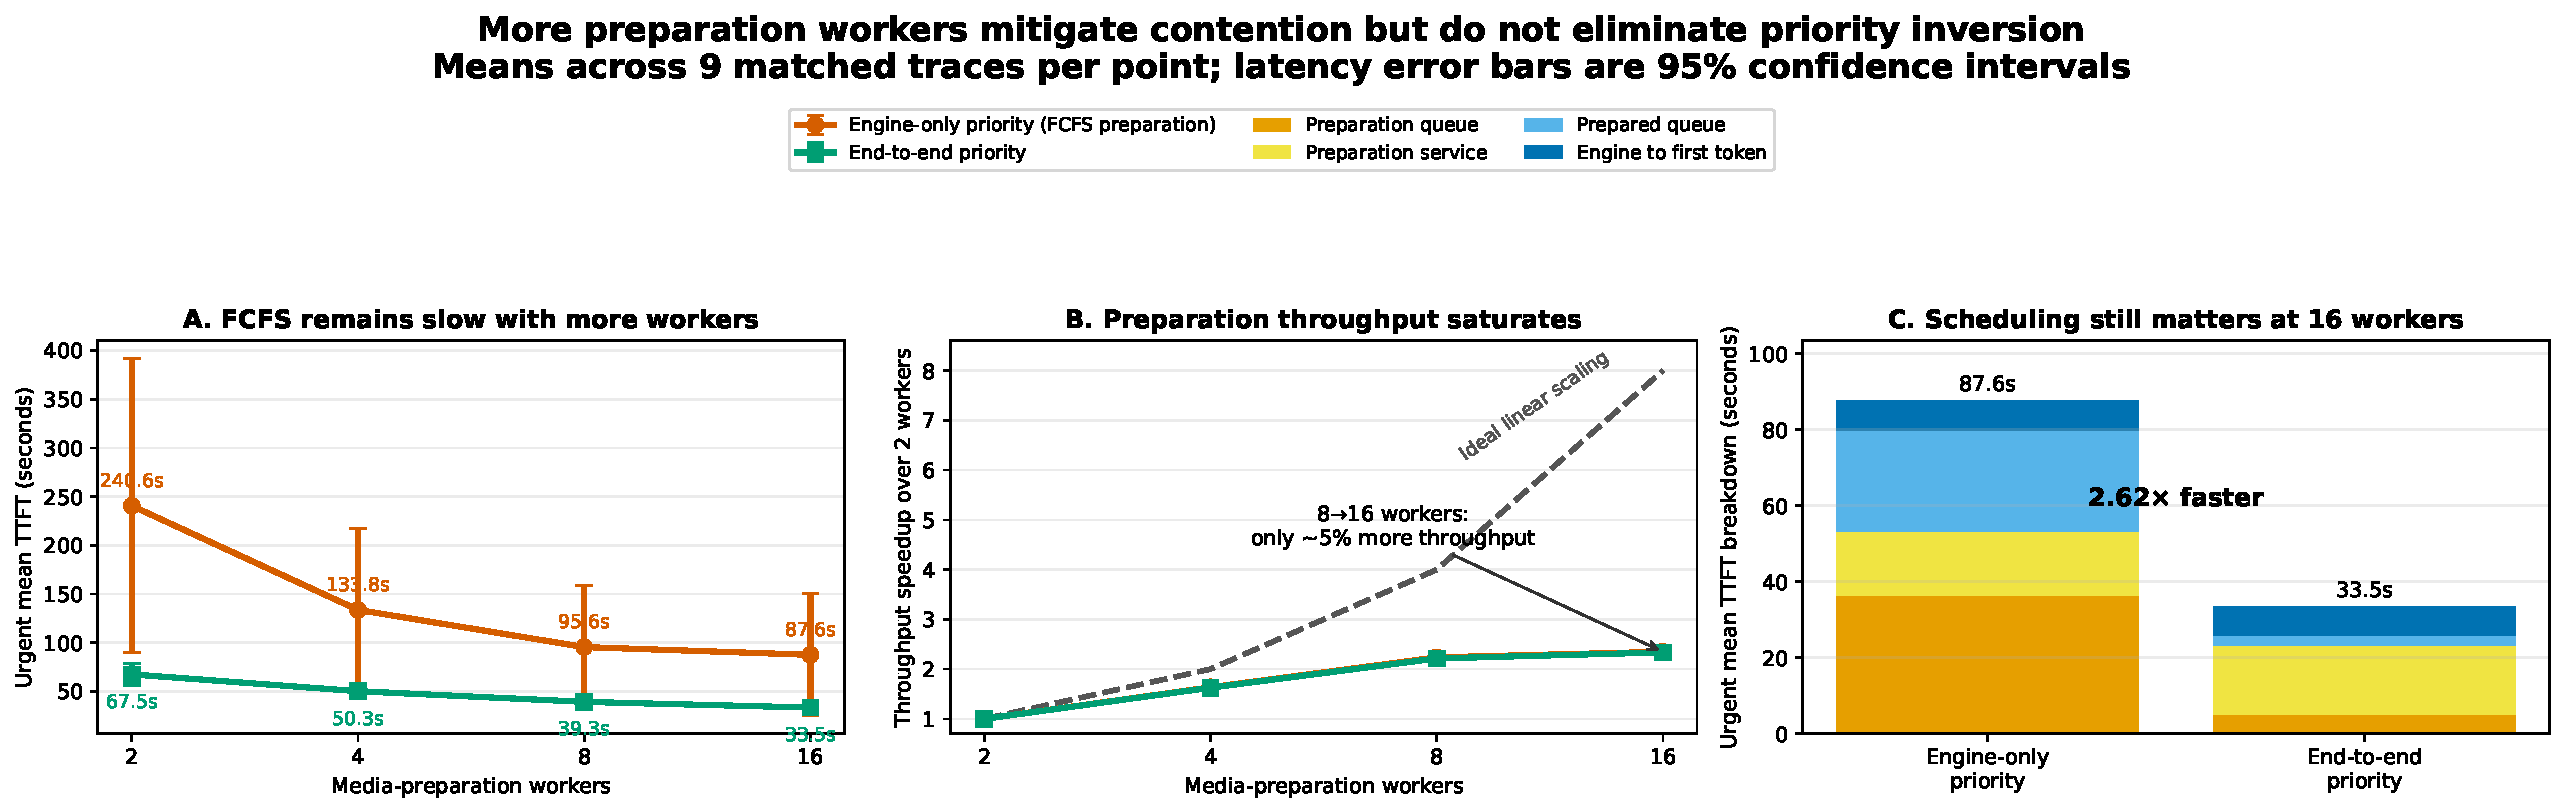
\includegraphics[width=\textwidth]
        {figures/preparation_scaling_wall.pdf}
    \caption{\textbf{Preparation-worker scaling.} More workers improve FCFS
    but do not eliminate upstream priority inversion. Error bars are 95\%
    confidence intervals across matched traces. Priority substantially lowers
    urgent TTFT while exposing the corresponding background-latency and
    reservation tradeoffs.}
    \Description{Three plots show urgent TTFT, background TTFT, and throughput
    as preparation workers increase from 2 to 16 for three policies.}
    \label{fig:worker-scaling}
\end{figure*}

\subsection{Inference Scale-Out Does Not Remove Shared Preparation}

Under fixed load, engine-only urgent TTFT remains 170.22, 162.23, and 159.79
seconds with one, two, and four replicas. End-to-end priority achieves 38.94,
37.24, and 32.13 seconds. Additional GPUs therefore do not eliminate the
shared upstream queue.

Under proportional load, offered requests increase from 80 to 160 and 320 as
replicas increase from one to four. Engine-only urgent TTFT grows from 22.74
to 226.19 seconds, whereas end-to-end priority limits it to 66.79 seconds.
Throughput plateaus because the four-worker preparation pool is shared by all
replicas. Scaling inference without scaling and scheduling preparation merely
moves the bottleneck upstream (Figure~\ref{fig:replica-scaling}).

\begin{figure*}[t]
    \centering
    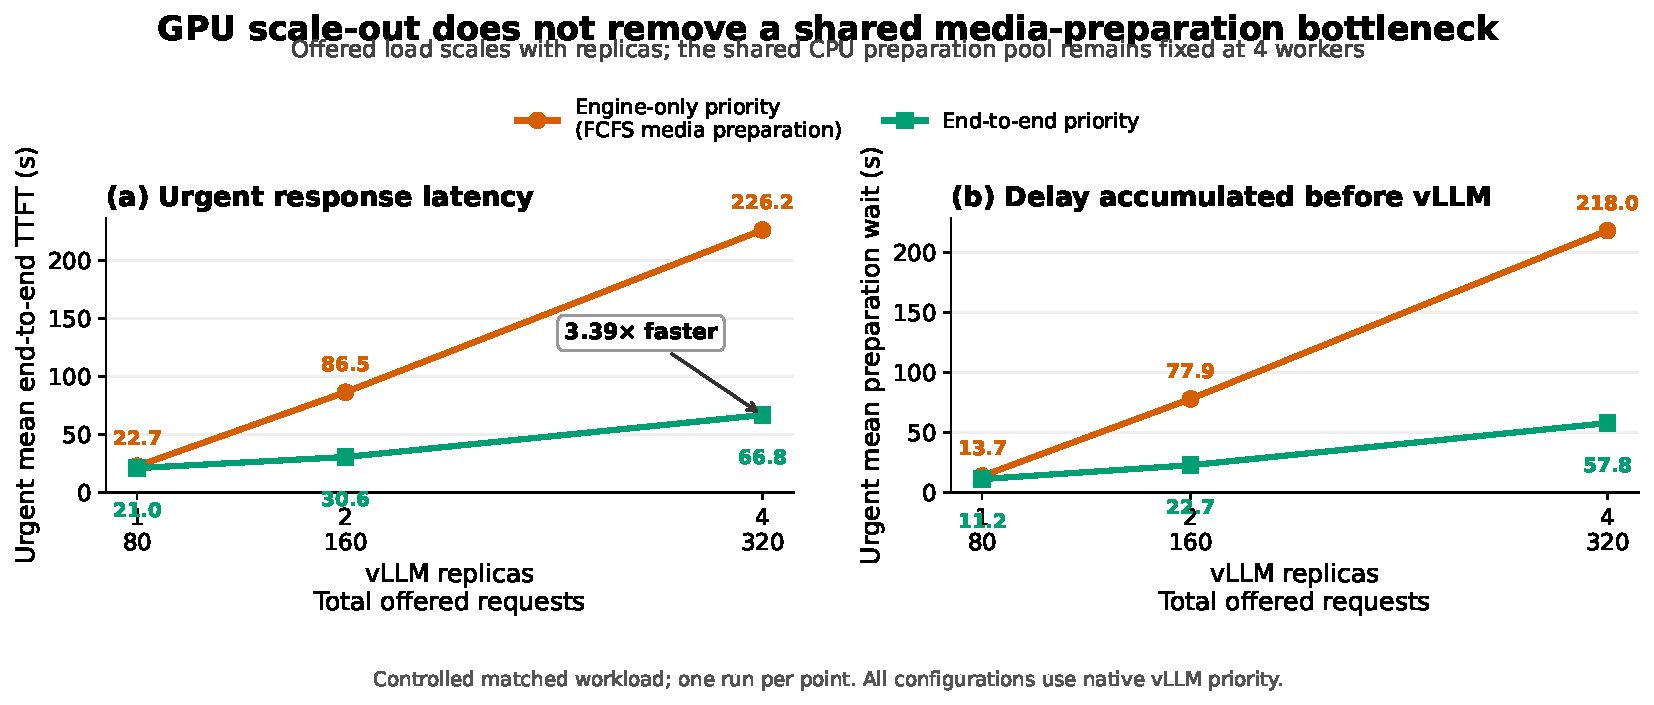
\includegraphics[width=\textwidth]
        {figures/replica_scaling_clean.pdf}
    \caption{\textbf{GPU scale-out does not remove a shared preparation
    bottleneck.} Offered load scales from 80 to 160 and 320 requests as the
    number of A40-backed vLLM replicas increases from one to four, while the
    shared CPU preparation pool remains fixed at four workers. Engine-only
    priority accumulates most of its urgent delay before vLLM admission.
    End-to-end priority reduces four-replica urgent mean TTFT from 226.2 to
    66.8 seconds (3.39$\times$). This is a controlled matched workload with
    one run per point; the figure does not show confidence intervals.}
    \Description{Two line charts compare engine-only and end-to-end priority
    as the number of vLLM replicas and offered requests increase. The first
    shows urgent end-to-end time to first token and the second shows urgent
    preparation-queue wait. Engine-only priority rises much faster in both
    panels.}
    \label{fig:replica-scaling}
\end{figure*}

\subsection{Sensitivity to Frame Budget}

At two frames per request, both policies achieve approximately 1.6-second
urgent mean TTFT because preparation is below capacity. At four frames,
end-to-end priority reduces urgent mean TTFT from 9.93 to 3.98 seconds, a
2.50$\times$ speedup. At eight frames, it reduces TTFT from 27.11 to 6.54
seconds, a 4.15$\times$ speedup. Priority becomes more valuable as aggregate
preparation contention grows, but its benefit is not limited to 128-frame
videos.

\begin{figure}[t]
    \centering
    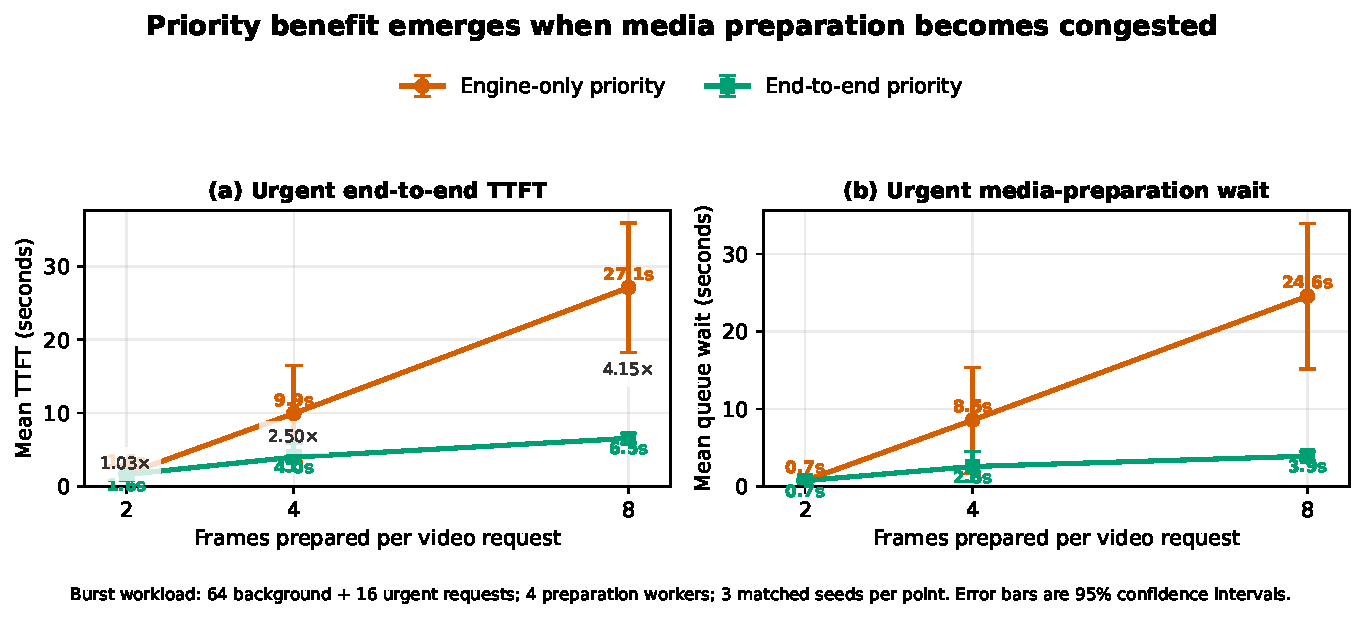
\includegraphics[width=\columnwidth]
        {figures/low_frame_priority_validation.pdf}
    \caption{\textbf{Priority benefit at small frame budgets.} The policies
    converge under an uncongested two-frame workload; priority becomes
    valuable as four- and eight-frame requests contend for preparation.}
    \Description{A plot compares urgent TTFT for engine-only and end-to-end
    priority at two, four, and eight frames.}
    \label{fig:low-frames}
\end{figure}

\subsection{Video Duration and Decoding Strategy}

Per-frame CPU seeking scales primarily with frame budget: its fitted
frame-count exponent is 1.00, while its duration exponent is only
$0.16\pm0.02$. In contrast, one-pass sequential CPU decoding has a duration
exponent of $1.06\pm0.04$ and a frame-count exponent of 0.21. Thus, video
duration is not universally proportional to preparation latency; the scaling
depends on how frames are accessed. Sequential decoding becomes expensive for
long videos, whereas seeking pays more directly for the number of requested
frames.

Naive sequential batched CPU decoding lowers throughput substantially in our
implementation, and the available NVDEC comparison contains unsupported or
failed inputs that can introduce survivor bias. We therefore treat decoding
backend optimization as complementary future work rather than attributing the
priority gains to a faster decoder.

\subsection{System Cost and Accuracy}

End-to-end priority shifts service toward urgent requests and can increase
background latency; reserved capacity makes this tradeoff stronger. In the
main comparison, ordinary priority preserves aggregate throughput, whereas
reservation lowers it. Answer quality does not explain the latency gain:
pooled successful urgent accuracy differs by only 0.35 percentage points
(58.68\% under engine-only priority and 59.03\% under end-to-end priority).

\section{Discussion and Limitations}
\label{sec:discussion}

\paragraph{Non-preemptive preparation.}
An urgent request can still wait for tasks already executing. The scheduler
overtakes queued work but does not interrupt active decoding. Decoder-aware
preemption may reduce this residual blocking but must account for discarded
work and restart cost.

\paragraph{Workload classes, tenant shares, and starvation.}
The system does not infer semantic urgency from video content. The operator
maps authenticated endpoints or execution contexts to foreground and
background classes and configures tenant weights. A tenant that labels every
request foreground still cannot consume another tenant's weighted share.
Aging provides progress within a tenant, while overload admission control is
still required when aggregate demand exceeds physical capacity.

\paragraph{Background cost.}
Priority improves urgent latency by delaying background work. Ordinary
priority is work-conserving and preserves throughput in our broad evaluation;
reserved capacity provides stronger protection but may reduce utilization.

\paragraph{Decoder optimization.}
Our contribution is scheduling, not a new decoder. Caching, NVDEC, faster
CPUs, storage improvements, and better frame selection reduce service time
and are complementary. No finite decoder speed eliminates the need for an
ordering policy once offered preparation work exceeds capacity.

\paragraph{Generality.}
The evaluation focuses on video question answering using one vision-language
model and A40 GPUs. Additional models, image and audio workloads, codecs, and
production traces remain future work. The completed tenant study uses
equal-weight tenants and a closed matched workload; sustained overload and
noisy-neighbor experiments are required before claiming bounded progress
under arbitrary continuous arrivals.

\section{Related Work}

\paragraph{LLM serving and engine scheduling.}
Continuous batching, iteration-level scheduling, preemption, and disaggregated
prefill and decode improve GPU utilization and responsiveness
~\cite{vllm,fastserve,andes,sarathiserve,distserve}. Our work addresses a
different boundary: requests blocked in external media preparation are not
yet visible to these engine mechanisms.

\paragraph{Multimodal serving and media optimization.}
Prior systems optimize multimodal preprocessing, token reduction, caching,
and media decoding. Such techniques reduce the amount or cost of preparation;
our scheduler determines which contending request receives that capacity
first. The approaches are complementary.

\paragraph{Priority and multi-stage systems.}
Priority inversion and head-of-line blocking are longstanding scheduling
problems. Fair LLM schedulers account for token service inside the model
engine, while agent and physical-AI systems schedule repeated generation and
external-execution rounds. Our setting exposes a complementary boundary:
one-shot multimodal requests consume fetch, decode, and transformation service
before they become model-ready. We use established virtual-service ideas but
extend the accounting and workload hierarchy across CPU preparation and GPU
admission rather than claiming a new single-resource fair-queueing primitive.

\section{Conclusion}

Engine-local scheduling begins too late to control the service received by a
multimodal request end to end. A tenant can be fairly served at the GPU yet
wait unfairly for CPU preparation, and a foreground request can lose most of
its latency objective before the engine observes it. Cross-stage virtual
service combined with within-tenant foreground priority reduces mean
completion latency by 3.94$\times$ relative to tenant fairness alone while
retaining nearly identical tenant isolation and throughput. The broader
lesson is that multimodal serving objectives must be accounted for at every
admission boundary that controls a finite, non-preemptive resource.

\bibliographystyle{ACM-Reference-Format}
\bibliography{references}

\end{document}
